\chapter{显微成像系统的检测实验}

% 通过搭建实验检测平台,对光学薄膜的表面缺陷通过进行观测检测验证。对照本 显微成像检测系统的原理框图搭建实验平台,通过显微成像实验平台,实验完成对照 明光源的位置设置、显微图像采集格式的设置、树莓派接口通信的调试,以及对图像 数据采集传输与控制进行测试,验证了光学薄膜表面缺陷检测系统具备可行性。

光学显微镜有景深浅这一特点,在高倍视场这一情况下这一特点尤其突出,当显微镜观察对象表面的不平整时,可能造成图像局部模糊,模糊的图像不利于对象观察的判断和目标识别和测量的正确性,如要取得清晰范围更大的图像,需要使用图像融合的方式进行图像处理。在整体的测试中,重点测试缺陷检测系统的可行性,查看最后的结果相关判定。

\section{薄膜表面缺陷检测测试}

\subsection{实验仪器介绍和安装}
该平台将分为两部分进行安装,一部分为实验装置的安装,后对系统烧录后进行驱动安装和图像测试,测试成功后安装对应的Django框架和相应程序。
实验仪器包括:CMOS摄像头,LED照明设备,显微镜头,树莓派版,显示器,HDMI线缆,以太网线缆,SD卡,外设设备等。
后续需要安装和设置的部分包括:raspbian系统,camera驱动,python安装,Django安装,网络配置,系统模块配置等。
\subparagraph{基础环境搭建}

先组装光学镜头部分,将之前选择好的显微镜头和CMOS摄像头通过CS口连接,后数据到ARM版卡的连接使用排线的方式。照明光源为LED的环状反射式照明,根据不同的薄膜透明度调节相应的亮度,进行数据的采集工作。之后将CMOS摄像头通过排线和ARM板的CSI-2接口进行连接,HDMI线缆将显示器与树莓派连接。

后进行基础的系统安装和配置。在Linux中使用dd命令将对应的镜像烧录到对应的SD卡的设备中,Windows可以使用NOOBS进行镜像的选择和启动。选择后可以进入命令行界面,进入配置的调试。在raspi-config中,选择配置对应的locale、module、sshd、overload等常见设置。后如选择进入命令行,则可用startx开启对应的桌面,也可在配置中默认启动。默认的账号和密码为pi和raspberry。对package进行更新和升级,安装vim-enchanced,调节对应的驱动安装,测试raspistill,raspivid和raspiyuv是否可用,后安装python,python3-picamera方便进行picamera的调用。可以安装python-picamera-docs进行查看。安装pypi,进行Django的安装。


\begin{figure}[h]
\centering
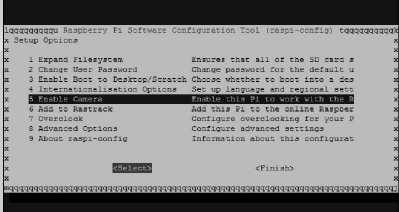
\includegraphics[width=0.7\linewidth]{Figure/rasp_4}
\caption{安装系统界面}
\label{fig:rasp_4}
\end{figure}

\subparagraph{软件系统设置(图片)}
%需要进行Django的安装和Server机的安装,
确认相关软件安装无误后,在localhost环境下进行测试,配置界面中调节好相应的jpeg的参数,包括帧数设定,时间间隔设定,存储位置设定,像素设定等。这里将帧数设定为每秒30帧,图像输出大小为4208x3120,每5秒拍摄一次,保存格式为jpeg。

搭建的实验系统平台如图 所示,连接显微镜头和 CMOS镜头后,在浏览器中输入localhost,进行相关的调节,并调节好显微镜焦距,观测镜片表面的薄膜。
%\subparagraph{使用方式解释说明}

\subsection{缺陷检测结果分析}
%在显微成像系统测试中,选取了实验室最常用的光学透镜的表面薄膜,观测了增 透膜和增反膜表面的缺陷程度,对表面出现的缺陷进行了分析。调整不同的光照方式, 对同一片增透膜进行了多次检测,以消除光照对检测误差的影响,通过采集不同的薄膜 显微图像,并对传输上来的图片进行了图像预处理,采用均值滤波算法滤除高斯噪声, 并对图像进行二值化处理,对采集的多幅图像进行比较选择,排除对焦不同等差异条 件。采集到的薄膜表面的显微图像原始数据。
%在上位机上对显微图像采用中值滤波进行图像降噪预处理,处理 结果如图所示。
%采用阈值分割处理算法对预处理过的图像做缺损检测处理,选定标准完整的薄膜 表面图像作为标准背景图,将显微系统采集到的带有缺损的薄膜表面图像与之对比, 对缺陷图像进行阈值分割处理,并截取放大显示识别出的典型的缺陷形状,选取记录 结果如下所示。

在系统测试中,选取了常用的光学透镜下的表面薄膜, ,观测了增 透膜和增反膜表面的缺陷程度,对表面出现的缺陷进行了分析。调整不同的光照方式,对相关的图片进行图像预处理,采用均值滤波算法过滤高斯噪声,并对图像进行二值化处理,其图像如图所示:
\begin{figure}[h]
\centering
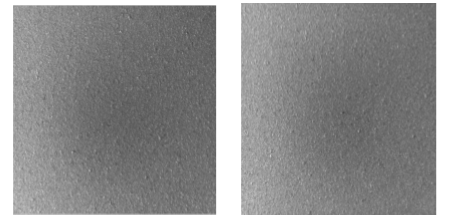
\includegraphics[width=0.7\linewidth]{Figure/ex_1}
\caption{示例图像}
\label{fig:ex_1}
\end{figure}

常见的缺陷记录在截取放大显示出的典型缺陷形状,如图所示,
\begin{figure}[h]
\centering
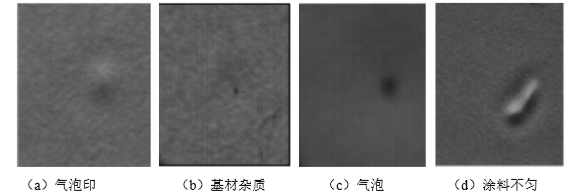
\includegraphics[width=0.7\linewidth]{Figure/ex_2}
\caption{主要缺陷图(ex)}
\label{fig:ex_2}
\end{figure}

在整体的测试过程中,通过B/S实现良好的跨机兼容性,先期通过1080p的30帧格式方式进行,测试相关选项条件并进行固定,通过CSI接口传到显示器调节。后期将用2160p的每5秒1帧的方式使用。整体通过TCP/IP协议将信息传递到对应的客户端,亦可借用有公网IP的宿主机作为服务器端达到公网查看的效果。此外,重点关注的高速实时的检测特点也得到了实现,同时实现了微型化智能化的特点。

%在对薄膜的缺陷检测实验中,CMOS 相机采集的速度在 1080P 格式下可以达到每秒 30 帧,通过 CSI 接口传到显示器,实现了对薄膜的实时检测和识别,还能够通过网口传 到局域网实现远程缺陷检测。相比传统的缺陷检测系统,整个缺陷检测系统硬件上采 用了性价比的 ARM 处理器,选用手机上常用的 CMOS 图像传感器 IMX135,并通过 CSI-2 串 行接口输出图像,实现了高速实时的检测特点。整个检测系统结构紧凑,Raspbian 操 作系统可更新升级,实现了微型化智能化的检测特点。
\section{本章小节}
本章搭建了基于ARM处理器的显微成像系统平台,通过选用不同光照强度的光源照明方式,测试了实验室的光学薄膜表面的缺陷,同时验证了该系统的实时检测性能,并对 采集的薄膜表面的图像进行处理,识别缺陷的类型和形状,达到了系统的总体设计要求。
